% \begin{frame}[fragile]{Chisel Today}
% \begin{itemize}
% \item whirlwind tour of chisel
% \item recents results and products
% \item update on upcoming release
% \item future research work
% \end{itemize}
% \end{frame}

\begin{frame}[fragile]
\frametitle{What is Chisel?}
\vfill
\begin{itemize}
\item {\bf Abstractly}: Chisel is a framework for {\it programmatically} generating circuitry.
\item {\bf Less Abstractly}: Chisel is a software library for creating and connecting circuit components to form a circuit graph.
\item {\bf Concretely}: Chisel is a DSL embedded in Scala for creating and connecting circuit components, with tools for simulation and translation to Verilog.
\end{itemize}
\vspace{3.5cm}
{\it\small * based on slides by my PhD student Patrick Li}
\end{frame}

\begin{frame}[fragile]
\frametitle{Chisel is a {\it Library}}
\begin{itemize}
\item Classes are provided for circuit components:
\begin{itemize}
\item \verb+Register()+
\item \verb+Adder()+
\item \verb+Multiplexor()+
\item \verb+Wire(name)+
\item \verb+Constant(name)+
\end{itemize}

\noindent
and \verb+new+ used to construct components and connect used to wire them together:
\begin{itemize}
\item \verb+new Register()+
\item ...
\item \verb+connect(input, output)+
\end{itemize}
\end{itemize}
\end{frame}

\begin{frame}[fragile]
\frametitle{What if Chisel was a Scala Library?}
\begin{columns}
\column{0.50\textwidth}
{\lstset{basicstyle={\tiny\ttfamily}}
\begin{scala}
def main (): Int = {
  // Create Components
  val reset       = new Wire("reset");
  val counter     = new Register("counter");
  val adder       = new Adder();
  val multiplexor = new Multiplexor();
  val one         = new UInt(1);
  val zero        = new UInt(0);

  // Connect Components
  connect(multiplexor.choice, reset);
  connect(multiplexor.in_a, zero.out);
  connect(multiplexor.in_b, adder.out);
  connect(counter.in, multiplexor.out);
  connect(adder.in_a, counter.out);
  connect(adder.in_b, one.out);

  // Produce Verilog
  generate_verilog(counter);
}
\end{scala}
}
\column{0.40\textwidth}
\begin{center}
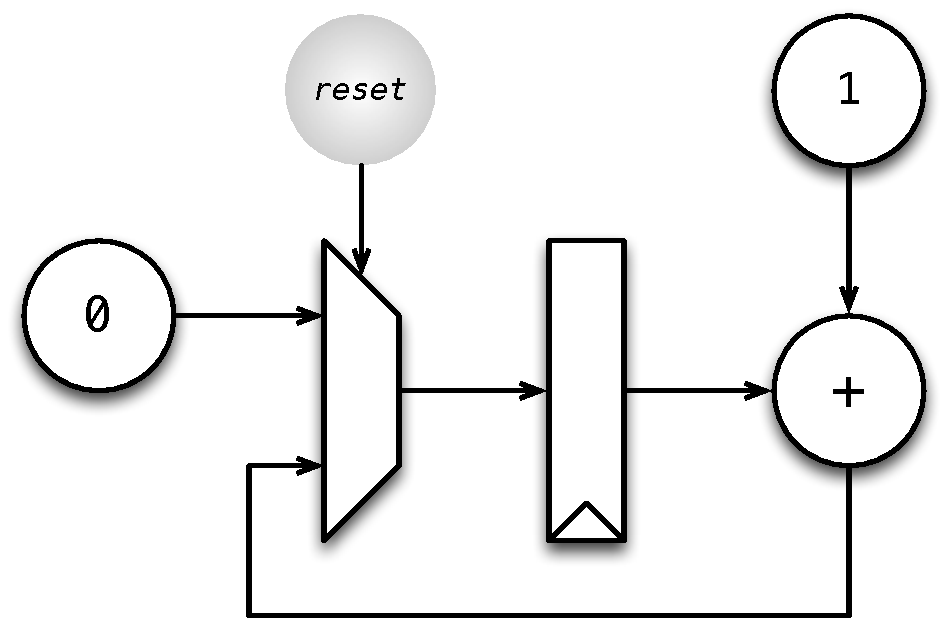
\includegraphics[width=0.9\textwidth]{figs/simple-counter.pdf}
\end{center}
\end{columns}
\end{frame}

\begin{frame}[fragile]
\frametitle{What if Chisel was a Scala Library?}
\begin{columns}
\column{0.50\textwidth}
{\lstset{basicstyle={\tiny\ttfamily}}
\begin{scala}
def main (): Int = {
  // Create Components
  val reset       = new Wire("reset");
  val counter     = new Register("counter");
  val adder       = new Adder();
  val multiplexor = new Multiplexor();
  val one         = new UInt(1);
  val zero        = new UInt(0);

  // Connect Components
  connect(multiplexor.choice, reset);
  connect(multiplexor.in_a, zero.out);
  connect(multiplexor.in_b, adder.out);
  connect(counter.in, multiplexor.out);
  connect(adder.in_a, counter.out);
  connect(adder.in_b, one.out);

  // Produce Verilog
  generate_verilog(counter);
}
\end{scala}
}
\column{0.40\textwidth}
\begin{center}
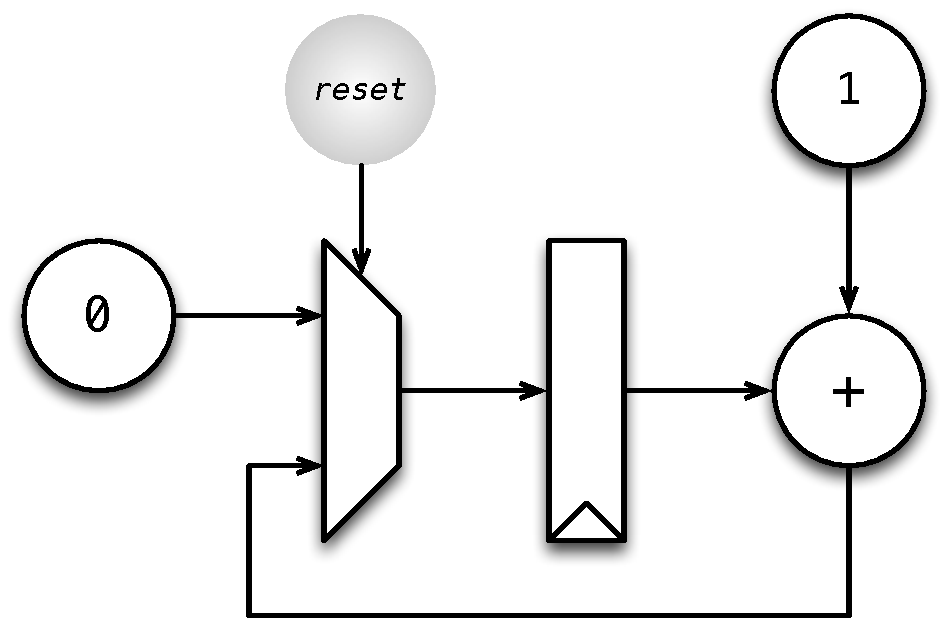
\includegraphics[width=0.9\textwidth]{figs/simple-counter.pdf}
\end{center}
\end{columns}
\begin{itemize}
\item using Scala to programmatically generate hardware
\item can use full power of Scala (loops, arrays, conditionals, ...)
\end{itemize}
\end{frame}

\begin{frame}[fragile]
\frametitle{What if Chisel was a Scala Library?}
\begin{columns}
\column{0.50\textwidth}
{\lstset{basicstyle={\tiny\ttfamily}}
\begin{scala}
def main (): Int = {
  // Create Components
  val reset       = new Wire("reset");
  val counter     = new Register("counter");
  val adder       = new Adder();
  val multiplexor = new Multiplexor();
  val one         = new UInt(1);
  val zero        = new UInt(0);

  // Connect Components
  connect(multiplexor.choice, reset);
  connect(multiplexor.in_a, zero.out);
  connect(multiplexor.in_b, adder.out);
  connect(counter.in, multiplexor.out);
  connect(adder.in_a, counter.out);
  connect(adder.in_b, one.out);

  // Produce Verilog
  generate_verilog(counter);
}
\end{scala}
}
\column{0.40\textwidth}
\begin{center}
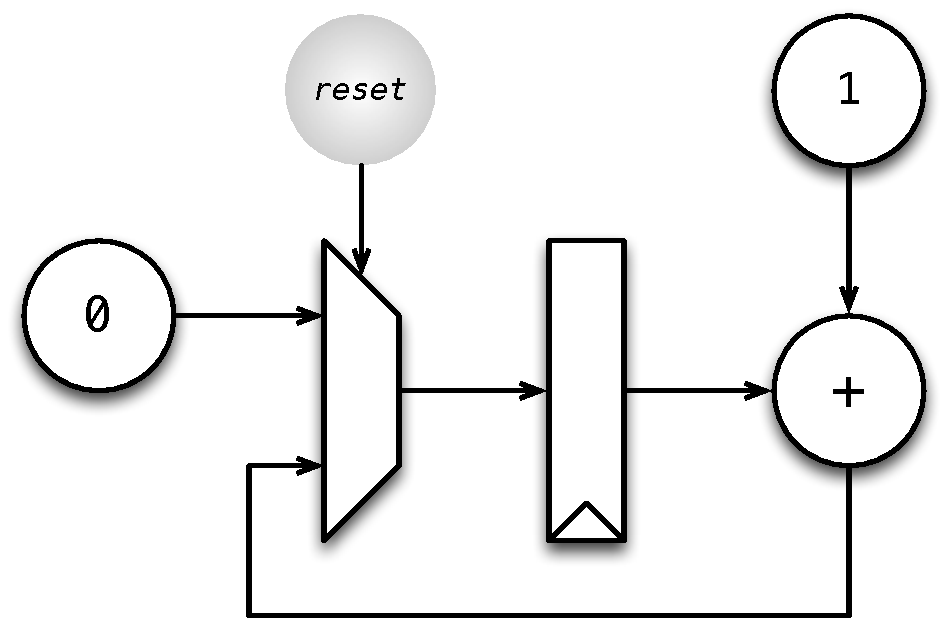
\includegraphics[width=0.9\textwidth]{figs/simple-counter.pdf}
\end{center}
\end{columns}
\begin{itemize}
\item but Scala is pretty Verbose, how can we do better?
\end{itemize}
\end{frame}

\begin{frame}[fragile]
\frametitle{Functional Composition of Adder}
\begin{columns}
\column{0.4\textwidth}
{\lstset{basicstyle={\tiny\ttfamily}}
\begin{scala}
def main (): Int = {
  // Create Components
  val reset       = new Wire("reset");
  val counter     = new Register("counter");
  val adder       = new Adder();
  val multiplexor = new Multiplexor();
  val one         = new UInt(1);
  val zero        = new UInt(0);

  // Connect Components
  connect(multiplexor.choice, reset);
  connect(multiplexor.in_a, zero.out);
  connect(multiplexor.in_b, adder.out);
  connect(counter.in, multiplexor.out);
  connect(adder.in_a, counter.out);
  connect(adder.in_b, one.out);

  // Produce Verilog
  generate_verilog(counter);
}
\end{scala}
}

\column{0.05\textwidth}
\begin{center}
$\Rightarrow$
\end{center}
\column{0.4\textwidth}

{\lstset{basicstyle={\tiny\ttfamily}}
\begin{scala}
def main (): Int = {
  // Create Components
  val reset       = new Wire("reset");
  val counter     = new Register("counter");
  val multiplexor = new Multiplexor();
  val one         = new UInt(1);
  val zero        = new UInt(0);

  // Connect Components
  connect(multiplexor.choice, reset);
  connect(multiplexor.in_a, zero.out);
  connect(multiplexor.in_b, 
          make_adder(one.out, counter.out));
  connect(counter.in, multiplexor.out);

  // Produce Verilog
  generate_verilog(counter);
}
\end{scala}
}
\end{columns}
\end{frame}

\begin{frame}[fragile]
\frametitle{Functional Composition of Multiplexor}
\begin{columns}
\column{0.4\textwidth}
{\lstset{basicstyle={\tiny\ttfamily}}
\begin{scala}
def main (): Int = {
  // Create Components
  val reset       = new Wire("reset");
  val counter     = new Register("counter");
  val multiplexor = new Multiplexor();
  val one         = new UInt(1);
  val zero        = new UInt(0);

  // Connect Components
  connect(multiplexor.choice, reset);
  connect(multiplexor.in_a, zero.out);
  connect(multiplexor.in_b, 
          make_adder(one.out, counter.out));
  connect(counter.in, multiplexor.out);

  // Produce Verilog
  generate_verilog(counter);
}
\end{scala}
}
\column{0.05\textwidth}
\begin{center}
$\Rightarrow$
\end{center}
\column{0.4\textwidth}
{\lstset{basicstyle={\tiny\ttfamily}}
\begin{scala}
def main (): Int = {
  // Create Components
  val reset   = new Wire("reset");
  val counter = new Register("counter");
  val one     = new UInt(1);
  val zero    = new UInt(0);

  // Connect Components
  connect(counter.in, 
    make_multiplexor(reset,
      zero.out
      make_adder(one.out, counter.out)));

  // Produce Verilog
  generate_verilog(counter);
}
\end{scala}
}
\end{columns}
\end{frame}

\begin{frame}[fragile]
\frametitle{Functional Composition of UInt Creation}
\begin{columns}
\column{0.4\textwidth}
{\lstset{basicstyle={\tiny\ttfamily}}
\begin{scala}
def main (): Int = {
  // Create Components
  val reset   = new Wire("reset");
  val counter = new Register("counter");
  val one     = new UInt(1);
  val zero    = new UInt(0);

  // Connect Components
  connect(counter.in, 
    make_multiplexor(reset,
      zero.out
      make_adder(one.out, counter.out)));

  // Produce Verilog
  generate_verilog(counter);
}
\end{scala}
}
\column{0.05\textwidth}
\begin{center}
$\Rightarrow$
\end{center}
\column{0.4\textwidth}
{\lstset{basicstyle={\tiny\ttfamily}}
\begin{scala}
def main (): Int = {
  // Create Components
  val reset   = new Wire("reset");
  val counter = new Register("counter");

  // Connect Components
  connect(counter.in, 
    make_multiplexor(reset,
      UInt(0),
      make_adder(UInt(1), counter.out)));

  // Produce Verilog
  generate_verilog(counter);
}
\end{scala}
}
\end{columns}
\end{frame}

\begin{frame}[fragile]
\frametitle{Overload Addition Operator}
\begin{columns}
\column{0.4\textwidth}
{\lstset{basicstyle={\tiny\ttfamily}}
\begin{scala}
def main (): Int = {
  // Create Components
  val reset   = new Wire("reset");
  val counter = new Register("counter");

  // Connect Components
  connect(counter.in, 
    make_multiplexor(reset,
      UInt(0),
      make_adder(UInt(1), counter.out)));

  // Produce Verilog
  generate_verilog(counter);
}
\end{scala}
}
\column{0.05\textwidth}
\begin{center}
$\Rightarrow$
\end{center}
\column{0.4\textwidth}
{\lstset{basicstyle={\tiny\ttfamily}}
\begin{scala}
def main (): Int = {
  // Create Components
  val reset   = new Wire("reset");
  val counter = new Register("counter");

  // Connect Components
  connect(counter.in, 
    make_multiplexor(reset,
      UInt(0),
      UInt(1) + counter.out));

  // Produce Verilog
  generate_verilog(counter);
}
\end{scala}
}
\end{columns}
\end{frame}

\begin{frame}[fragile]
\frametitle{Introduce Connect Infix Operator}
\begin{columns}
\column{0.4\textwidth}
{\lstset{basicstyle={\tiny\ttfamily}}
\begin{scala}
def main (): Int = {
  // Create Components
  val reset   = new Wire("reset");
  val counter = new Register("counter");

  // Connect Components
  connect(counter.in, 
    make_multiplexor(reset,
      UInt(0),
      UInt(1) + counter.out));

  // Produce Verilog
  generate_verilog(counter);
}
\end{scala}
}
\column{0.05\textwidth}
\begin{center}
$\Rightarrow$
\end{center}
\column{0.4\textwidth}
{\lstset{basicstyle={\tiny\ttfamily}}
\begin{scala}
def main (): Int = {
  // Create Components
  val reset   = new Wire("reset");
  val counter = new Register("counter");

  // Connect Components
  counter.in :=
    make_multiplexor(reset,
      UInt(0),
      UInt(1) + counter.out);

  // Produce Verilog
  generate_verilog(counter);
}
\end{scala}
}
\end{columns}
\end{frame}

\begin{frame}[fragile]
\frametitle{Automatically Create Multiplexors}
\begin{columns}
\column{0.4\textwidth}
{\lstset{basicstyle={\tiny\ttfamily}}
\begin{scala}
def main (): Int = {
  // Create Components
  val reset   = new Wire("reset");
  val counter = new Register("counter");

  // Connect Components
  counter.in :=
    make_multiplexor(reset,
      UInt(0),
      UInt(1) + counter.out);

  // Produce Verilog
  generate_verilog(counter);
}
\end{scala}
}
\column{0.05\textwidth}
\begin{center}
$\Rightarrow$
\end{center}
\column{0.4\textwidth}
{\lstset{basicstyle={\tiny\ttfamily}}
\begin{scala}
def main (): Int = {
  // Create Components
  val reset   = new Wire("reset");
  val counter = new Register("counter");

  // Connect Components
  when (reset) {
    counter.in := UInt(0);
  } .otherwise {
    counter.in := UInt(1) + counter.out;
  }

  // Produce Verilog
  generate_verilog(counter);
}
\end{scala}
}
\end{columns}
\end{frame}

\begin{frame}[fragile]
\frametitle{Grab Names of Wires Directly}
\begin{columns}
\column{0.4\textwidth}
{\lstset{basicstyle={\tiny\ttfamily}}
\begin{scala}
def main (): Int = {
  // Create Components
  val reset   = new Wire("reset");
  val counter = new Register("counter");

  // Connect Components
  when (reset) {
    counter.in := UInt(0);
  } .otherwise {
    counter.in := UInt(1) + counter.out;
  }

  // Produce Verilog
  generate_verilog(counter);
}
\end{scala}
}
\column{0.05\textwidth}
\begin{center}
$\Rightarrow$
\end{center}
\column{0.4\textwidth}
{\lstset{basicstyle={\tiny\ttfamily}}
\begin{scala}
def main (): Int = {
  // Create Components
  val reset   = new Wire();
  val counter = new Register();

  // Connect Components
  when (reset) {
    counter.in := UInt(0);
  } .otherwise {
    counter.in := UInt(1) + counter.out;
  }

  // Produce Verilog
  generate_verilog(counter);
}
\end{scala}
}
\end{columns}
\end{frame}

\begin{frame}[fragile]
\frametitle{Abstract Counter}
\begin{columns}
\column{0.4\textwidth}
{\lstset{basicstyle={\tiny\ttfamily}}
\begin{scala}
def main (): Int = {
  // Create Components
  val reset   = new Wire();
  val counter = new Register();

  // Connect Components
  when (reset) {
    counter.in := UInt(0);
  } .otherwise {
    counter.in := UInt(1) + counter.out;
  }

  // Produce Verilog
  generate_verilog(counter);
}
\end{scala}
}
\column{0.05\textwidth}
\begin{center}
$\Rightarrow$
\end{center}
\column{0.4\textwidth}
{\lstset{basicstyle={\tiny\ttfamily}}
\begin{scala}
def make_counter(reset: Boolean) = {
  val counter = new Register();
  when (reset) {
    counter.in := UInt(0);
  } .otherwise {
    counter.in := UInt(1) + counter.out;
  }
  counter
}

def main (): Int = {
  // Create Components
  val reset   = new Wire();
  val counter = make_counter(reset);

  // Produce Verilog
  generate_verilog(counter);
}
\end{scala}
}
\end{columns}
\end{frame}

\begin{frame}[fragile]
\frametitle{Make Reset Implicit}
\begin{columns}
\column{0.4\textwidth}
{\lstset{basicstyle={\tiny\ttfamily}}
\begin{scala}
def make_counter(reset: Boolean) = {
  val counter = new Register();
  when (reset) {
    counter.in := UInt(0);
  } .otherwise {
    counter.in := UInt(1) + counter.out;
  }
  counter
}

def main (): Int = {
  // Create Components
  val reset   = new Wire();
  val counter = make_counter(reset);

  // Produce Verilog
  generate_verilog(counter);
}
\end{scala}
}
\column{0.05\textwidth}
\begin{center}
$\Rightarrow$
\end{center}
\column{0.4\textwidth}
{\lstset{basicstyle={\tiny\ttfamily}}
\begin{scala}
def make_counter() = {
  val counter = new Register();
  when (reset) {
    counter.in := UInt(0);
  } .otherwise {
    counter.in := UInt(1) + counter.out;
  }
  counter
}

def main (): Int = {
  // Create Components
  val reset   = new Wire();
  val counter = 
    withReset(reset) {
      make_counter(reset);
    }
  // Produce Verilog
  generate_verilog(counter);
}
\end{scala}
}
\end{columns}
\end{frame}

\begin{frame}[fragile]
\frametitle{Looks ``Behavioral'' but ...}
\begin{columns}
\column{0.50\textwidth}
{\lstset{basicstyle={\tiny\ttfamily}}
\begin{scala}
def make_counter() = {
  val counter = new Register();
  when (reset) {
    counter.in := UInt(0);
  } .otherwise {
    counter.in := UInt(1) + counter.out;
  }
  counter
}

def main (): Int = {
  // Create Components
  val reset   = new Wire();
  val counter = 
    withReset(reset) {
      make_counter(reset);
    }
  // Produce Verilog
  generate_verilog(counter);
}
\end{scala}
}
\column{0.40\textwidth}
\begin{center}
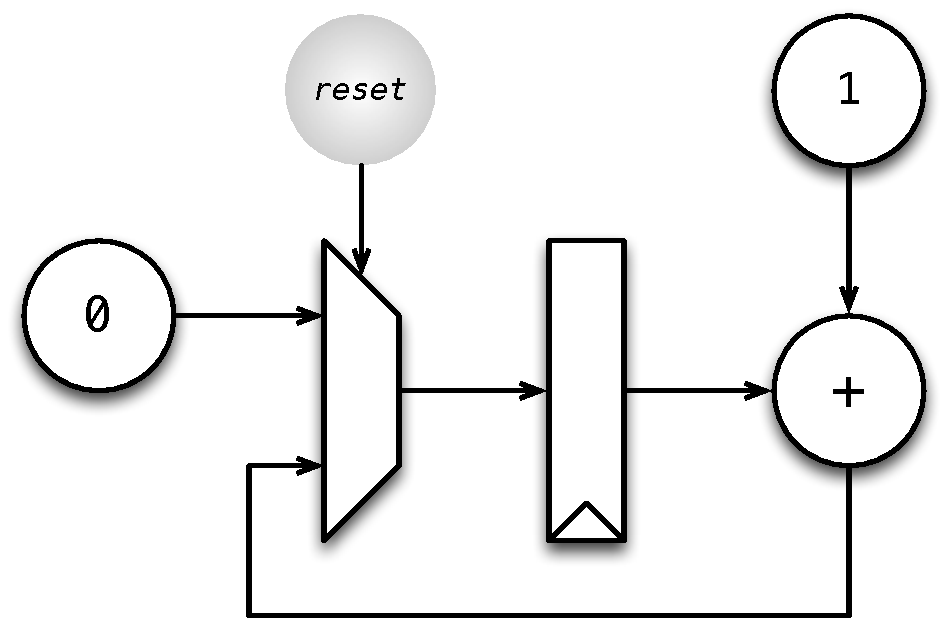
\includegraphics[width=0.9\textwidth]{figs/simple-counter.pdf}
\end{center}
\end{columns}
\begin{itemize}
\item every construct actually creates a concrete circuit
\item know cost of everything
\item layered and can choose level of abstraction
\end{itemize}
\end{frame}

\begin{frame}[fragile]{Hosting Language Ingredients}
Crucial
\begin{itemize}
\item Type Inference
\item Infix Operator Overloading
\item Lightweight Closures
\item Dynamic Scoping
\item Introspection or Simple Macros
\item Functional Programming
\end{itemize}
\vspace{0.5cm}
Even Better with
\begin{itemize}
\item Object Orientation
\item Powerful Macros
\end{itemize}
\end{frame}

\begin{frame}[fragile]{Synthesizable By Construction}
Well formed Chisel graphs are synthesizable.
\begin{columns}
\column{0.6\textwidth}
\begin{itemize}
\item Use small number of basic nodes
\begin{itemize}
\item simple semantics
\item easy to synthesize
\end{itemize}
\item During construction check that
\begin{itemize}
\item types, directions and widths match
\item there are no combinational loops
\end{itemize}
\end{itemize}
\column{0.3\textwidth}
\begin{center}
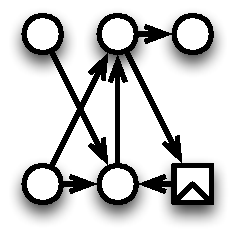
\includegraphics[width=0.9\textwidth]{figs/synthesizable.pdf}
\end{center}
\end{columns}
\vspace{1cm}
\begin{itemize}
\item {\color{red}If it passes these checks then it's synthesizable}
\end{itemize}
\end{frame}

\begin{frame}[fragile]{Hardware Language Approaches}
% \begin{columns}
% \column{0.45\textwidth}
\begin{itemize}
\item {\color{magenta}behavioral} -- high level language compiled to verilog
\begin{itemize}
\item examples: C, Lime, CHP, Esterel, BlueSpec
\end{itemize}
\item {\color{orange}simulation} -- simulation language with synthesizable subset
\begin{itemize}
\item examples: Verilog, System Verilog, SystemC, myHDL
\end{itemize}
\item {\color{green}construction} -- programmatically construct circuits
\begin{itemize}
\item examples: Chisel, Lava
\end{itemize}
\end{itemize}
% \column{0.45\textwidth}
% \begin{center}
% 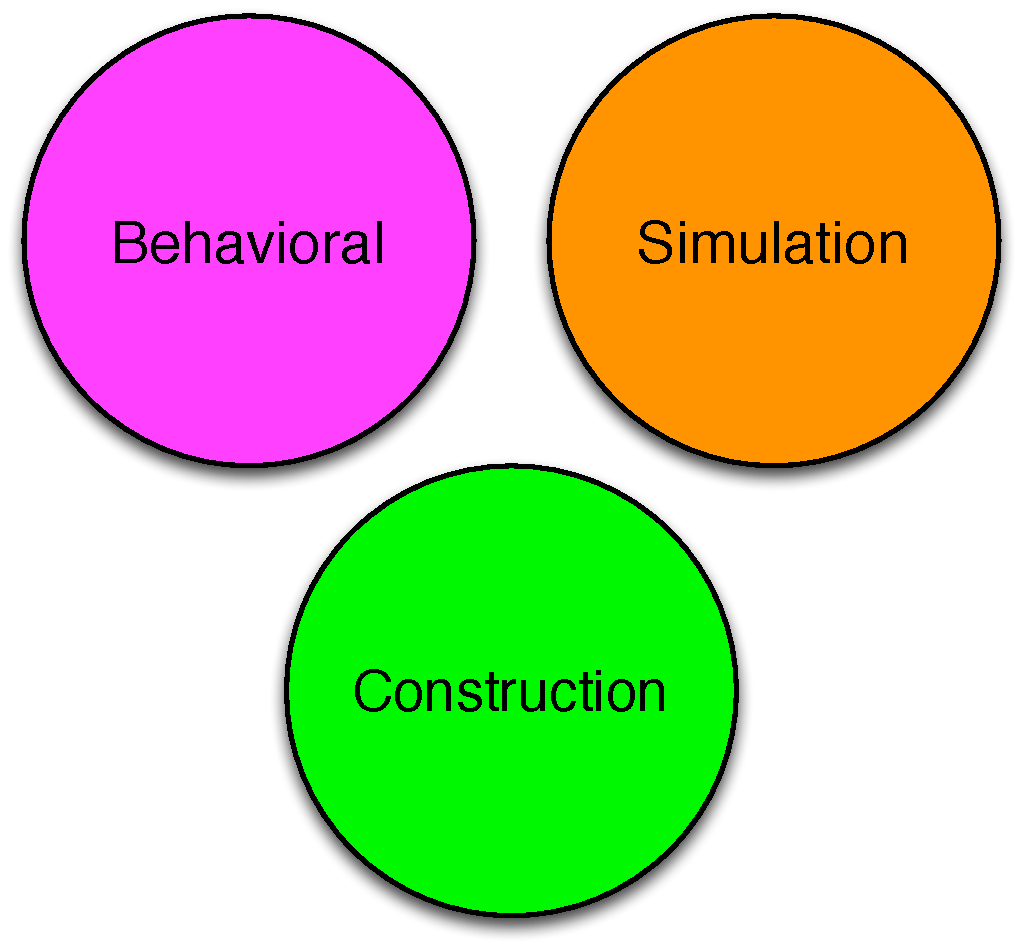
\includegraphics[width=1.0\textwidth]{figs/hdls.pdf} 
% \end{center}
% \end{columns}
\end{frame}

\begin{frame}[fragile]{Hardware Language Comparisons}
\begin{small}
\begin{center}
\begin{tabular}{|r|c|c|c|}
\hline
{\bf name} & {\bf example} & {\bf pros} & {\bf cons} \\ 
\hline
{\color{magenta}behavioral} & C-to-gates & high level & unpredictable \\
 &  &  & QoR \\
\hline
{\color{orange}simulation} & Verilog & flexible & synthesizable? + \\
 &  &  & low abstraction \\
\hline
{\color{green}construction} & Chisel & metaprogramming + & two levels + \\
 &  & predictable QoR + & blemishes \\
 &  &  synthesizable QoR &  \\
\hline
\end{tabular}
\end{center}
\end{small}

\begin{columns}
\column{0.4\textwidth}
\begin{center}
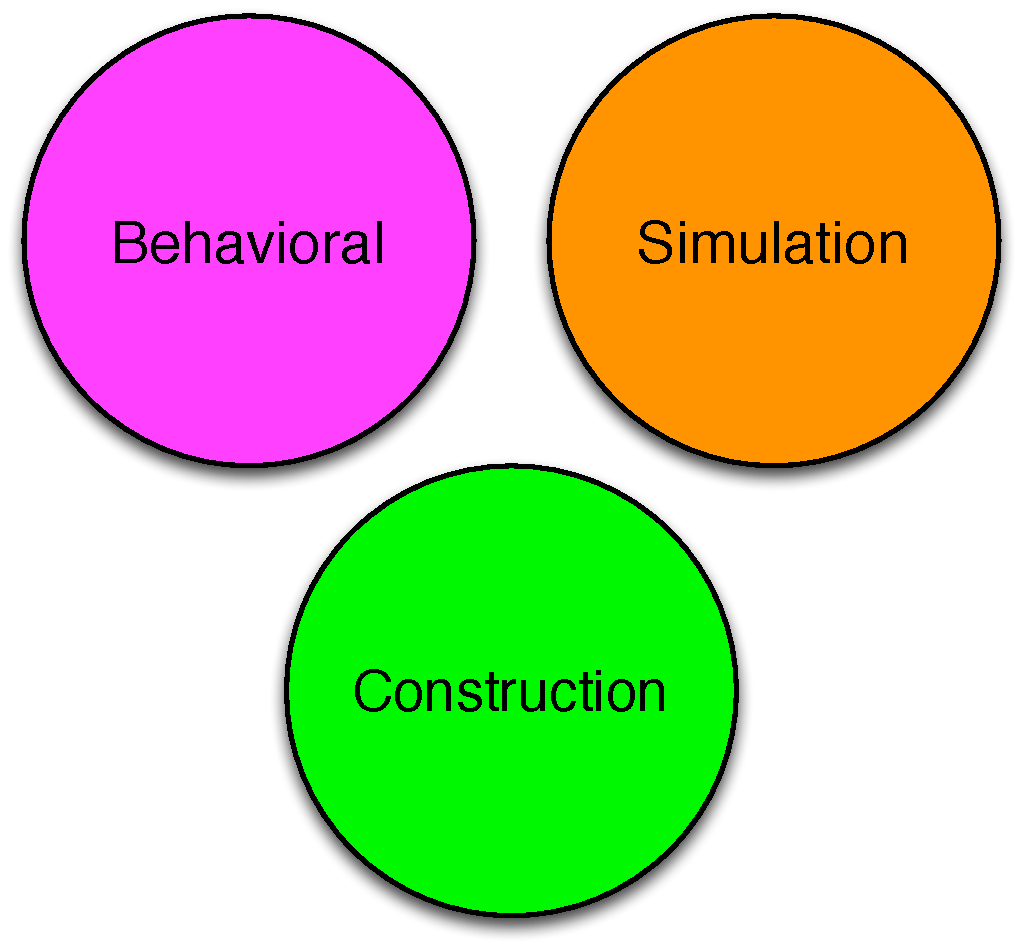
\includegraphics[width=0.8\textwidth]{figs/hdls.pdf} 
\end{center}
\column{0.5\textwidth}
Chisel
\begin{itemize}
\item is {\bf not} Scala to Verilog
\item produces circuits that are synthesizable by construction
\item permits simulation by driving synthesized design
\end{itemize}
\end{columns}
\end{frame}
